\documentclass[10pt]{article}
\title{Using Generative Adversarial Networks (GANs) to Generate Original Music}
\author{Guy Coop \footnote{
gtc434@student.bham.ac.uk | ID:1447634}\\ 
Supervisor: Per Kristian Lehre
}

%----------------------------------------
%packages
\usepackage[margin=3cm]{geometry}
\usepackage{amssymb}
\usepackage{cite}
\usepackage{graphicx}
\usepackage{float}

\usepackage{lipsum}

\begin{document}
\maketitle
\pagenumbering{gobble}
%----------------------------------------
%begin abstract
\section*{Abstract}
PLACEHOLDER TEXT\\
\lipsum[5]
\newpage

%----------------------------------------
%contents pages
\pagenumbering{roman}
\tableofcontents
\newpage
\listoffigures
\listoftables
\newpage

%----------------------------------------
%begin introduction
\pagenumbering{arabic}
\section{Introduction}
Generative Adversarial Networks (GANs) were first introduced in 2014 by Goodfellow et al. \cite{Goodfellow2014} and have since formed a foundation for a new method of unsupervised learning. In which two "opponents" are competing in the form of a zero-sum game to facilitate the training of networks without a specially designed loss function. This method has shown great success in creative tasks, often producing results that are superficially indistinguishable from human produced media. \\
This paper will attempt to apply this method to the relatively unexplored area of music generation, using a similar method to that of Elgammal et al. \cite{Elgammal2017} in which the loss function was partially dependant on a classifier network that determined the period of the art. In the same way, the loss function used in this paper will be partially dependent on being unable to classify the genre of the music, this should result in music that appears novel as it is a strict subset of a completely novel genre of music. \\
 


%----------------------------------------
%begin literature review
\section{Background to Theory}
\subsection{Generative Adversarial Networks}
Generative Adversarial Networks \cite{Goodfellow2014} use two agents competing in the form of a zero-sum game to try and complete creative tasks without the need to design a highly complex loss function. A very generic model can also be used for a number of different applications without needing to be redesigned due to the nature of the system. A simple description of the model is given by the following analogy: \\
A currency {\it forger} and a {\it policeman} take the place of the two competing agents. The {\it forger's} goal is to produce passable fake currency, and the {\it policeman's} goal is to differentiate fake and real currency. (For the sake of this example, it is important to pretend that the policeman has had no training, and the forger has never seen any real currency). The {\it forger} attempts to produce currency and put it into circulation, the {\it policeman} always finds it with the rest of the normal currency, and he looks at each note and declares it either real or fake. At the end of a round, the both the {\it policeman} and the {\it forger} are told how many forged notes were sucessfully detected, from this, the {\it policeman} becomes better at detecting forged notes, and the {\it forger} becomes better at forging realistic notes.

\subsection{Recurrent Neural Networks}
PLACEHOLDER \cite{Zaremba2014} \cite{Shi2017} \cite{Lipton2015}

\subsection{Convolutional Neural Networks}
PLACEHOLDER \cite{Radford2015}

\subsection{Related Work}
In the paper by Elgammal et al. \cite{Elgammal2017} great importance is placed on creating novelty without straying too far from accepted norms, this theory is motivated by the theory of Wilhelm Max Wundt. \cite{Wundt1874} this theory can be easily shown with the Wundt Curve (Figure \ref{fig:wundt_curve})

\begin{figure}[H]
\centering
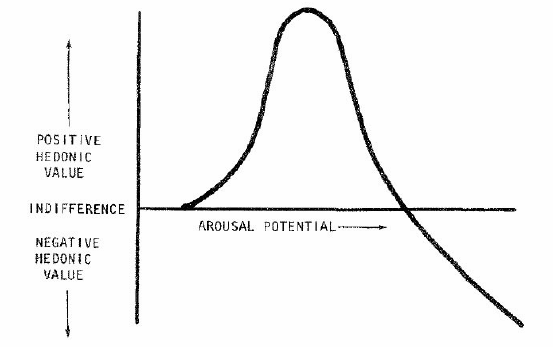
\includegraphics[scale=0.8]{wundt_curve}
\caption[Wundt curve for measuring arousal]{\label{fig:wundt_curve} The Wundt curve, used for measuring arousal potential, showing how hedonic response can decrease once novelty increases beyond a certain point}
\end{figure}

It is important to note that on the Wundt Curve, hedonic value decreases after a certain arousal potential. This implies that if the "creativity" of the media increases beyond a certain point it is no longer reacted to positively and instead becomes too abstract for humans to appreciate. \\

PLACEHOLDER Midi-Net \cite{Yang2017} MUSE-GAN \cite{Dong2017}


%----------------------------------------
%begin explaination of my project design
\section{System Design}


%----------------------------------------
%begin explaination of my project implementation
\section{Implementation of the Project}
\subsection{Data Preprocessing}
Explaination of the pre-processing done on the midi files

\subsection{Proof of concept}
When implementing a project of this scale, a proof of concept "toy" project is often useful to help verify that some of the subsytems are working without needing to implement the entire system. Details of the design, implementation, and testing of this proof of concept model are given below.
\subsubsection{Design}
This model uses a GAN, where both the discriminator and the generator are simple feed forward neural networks. The network diagram is given in Figure \ref{fig:toy_proj}

\begin{figure}[H]
\centering
%\includegraphics[scale=0.8]{•}
\caption[System diagram for proof of concept model]{\label{fig:toy_proj} A system diagram showing the network design for the proof-of-concept model}
\end{figure}

\subsubsection{Implementation}

\subsubsection{Testing and Experimentation}
%----------------------------------------
%begin explaination of my experimentation
\section{Experimentation}

%----------------------------------------
%bibliography
\newpage
\bibliography{full_bibliography}
\bibliographystyle{alpha}

\end{document}